En aquest capítol es detalla l'arquitectura del sistema i el disseny de les aplicacions desenvolupades.
\section{Arquitectura del sistema}
	L'arquitectura del sistema està formada per tres parts diferenciades: Un smartphone (aplicació usuari), un servidor i el robot. A continuació podeu veure un esquema de l'arquitectura i l'explicació
	de cada una de les parts.\\
	\begin{figure}[H]
		\centering
		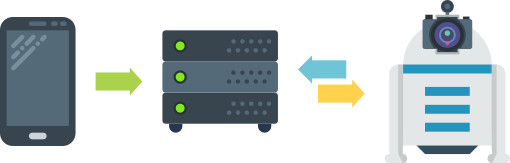
\includegraphics[width=0.7\textwidth]{images/arquitectura}
		\caption{Arquitectura del sistema}
	\end{figure}
	\vspace{0.05cm}
	\begin{itemize}
		\item{\textbf{Smartphone:} Permet a l'usuari seleccionar una regió en una imatge (de la càmera o la galeria) i l'envia al servidor.}
		\item{\textbf{Servidor:} Rep les imatges de l'smartphone i el robot i s'encarrega de fer el matching per obtenir el moviment necessari del robot.}
		\item{\textbf{Robot:} Envia les imatges capturades al servidor i espera rebre les ordres per desplaçar-se i girar.\\}
	\end{itemize}
	El treball es centrarà en la part del servidor i segons el temps disponible es realitzarà la comunicació entre el servidor i l'aplicació per a smartphones.

\section{Aplicació de proves}
	Inicialment es desenvoluparà una aplicació per realitzar les diverses proves sense interfície gràfica, que simplement mostrarà el resultat obtingut del matching. Més endavant, pero, s'inclourà una
	interfície mínima que ens permetrà escollir les imatges a tractar i la regió d'interès (punt de destí).
	\subsubsection{Selecció de les imatges}
		Per seleccionar les imatges s'utilitzarà Tkinter, una GUI estàndard de Python.\\
		\begin{figure}[H]
			\centering
			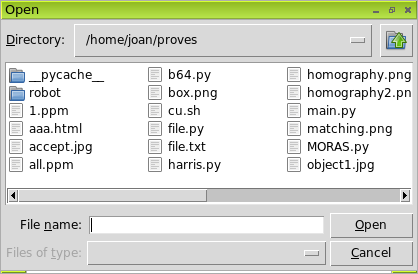
\includegraphics[width=0.5\textwidth]{images/fs}
			\caption{Selecció de les imatges}
		\end{figure}

	\subsubsection{Selecció de la regió d'interès}
		Per poder escollir el punt de destí del robot, l'usuari haurà de seleccionar una regió d'interès en una imatge. Això es farà de manera molt senzilla, fent una selecció amb el ratolí.
		Un cop realitzada la selecció, l'usuari tindrà la opció de refer-la (simplement seleccionant de nou) o d'acceptar-la pulsant la tecla "c".\\
		\begin{figure}[H]
			\centering
			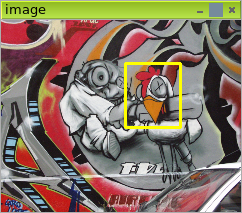
\includegraphics[width=0.5\textwidth]{images/selection}
			\caption{Selecció de la regió d'interès}
		\end{figure}
\newpage
\section{Disseny de l'aplicació mòbil}
	La interfície de l'aplicació mòbil és també molt simple. Inicialment trobarem un menú que ens permetrà accedir a les funcionalitats del programa, donant-nos a escollir entre les següents opcions:
	\begin{itemize}
		\item{\textbf{Fer una foto}}
		\item{\textbf{Seleccionar una imatge}}
		\item{\textbf{Opcions}}
	\end{itemize}
	\begin{figure}[H]
		\centering
		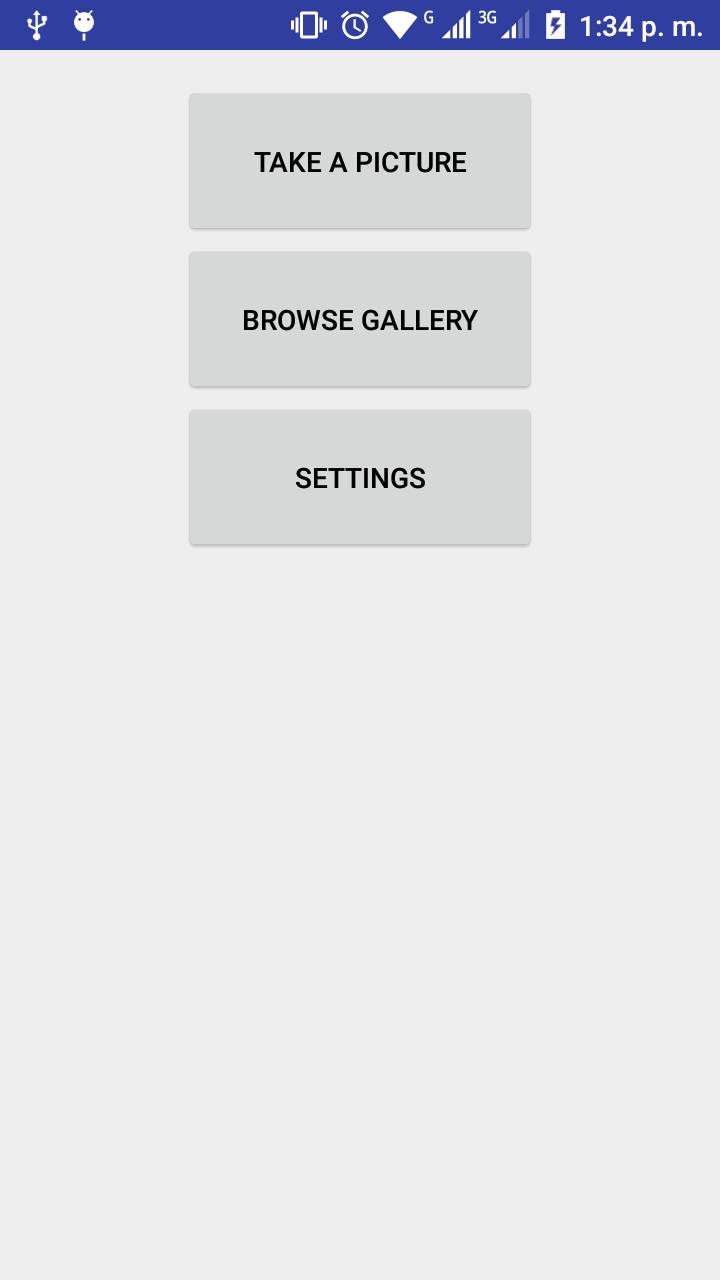
\includegraphics[width=0.5\textwidth]{images/menu}
		\caption{App - Menú}
	\end{figure}
	\subsubsection{Fer una foto}
		Permet a l'usuari fer una foto amb la càmera del dispositiu, per desprès seleccionar la regió d'interès.\\
		\begin{figure}[H]
			\begin{minipage}{6in}
				\centering
				\raisebox{-0.5\height}{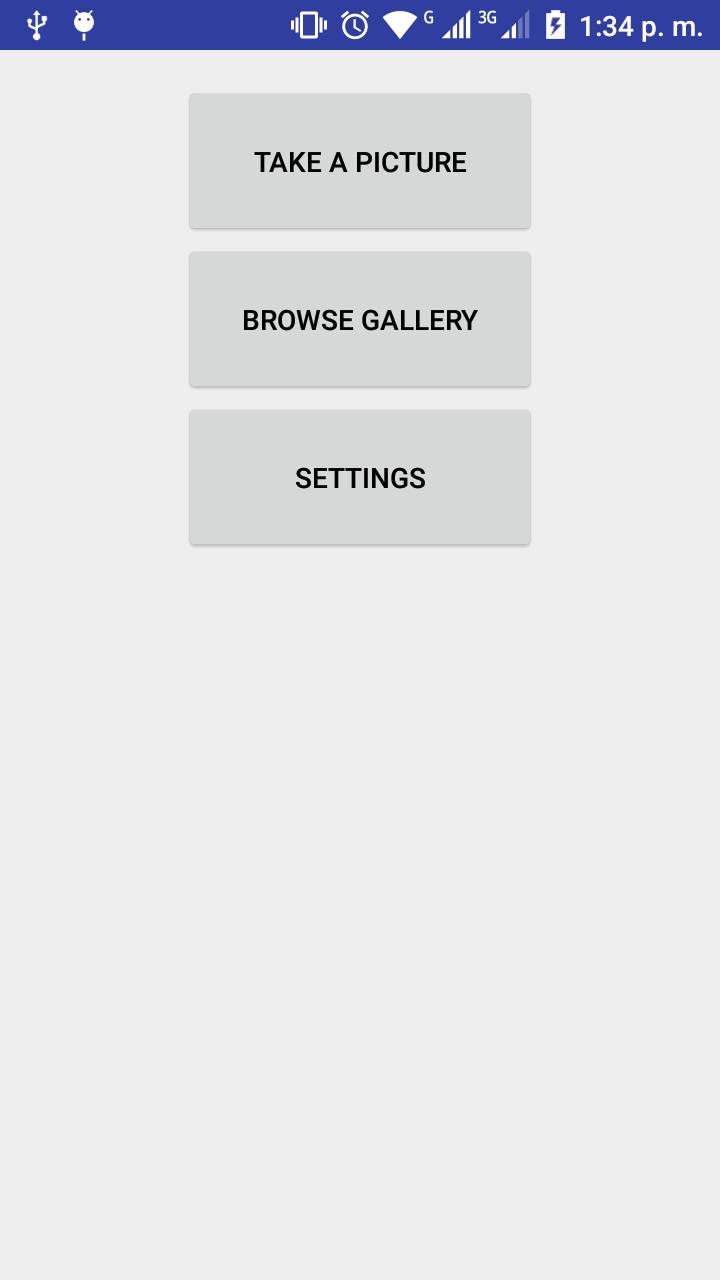
\includegraphics[width=0.4\textwidth]{images/menu}}
				\hspace*{.2in}
				\raisebox{-0.5\height}{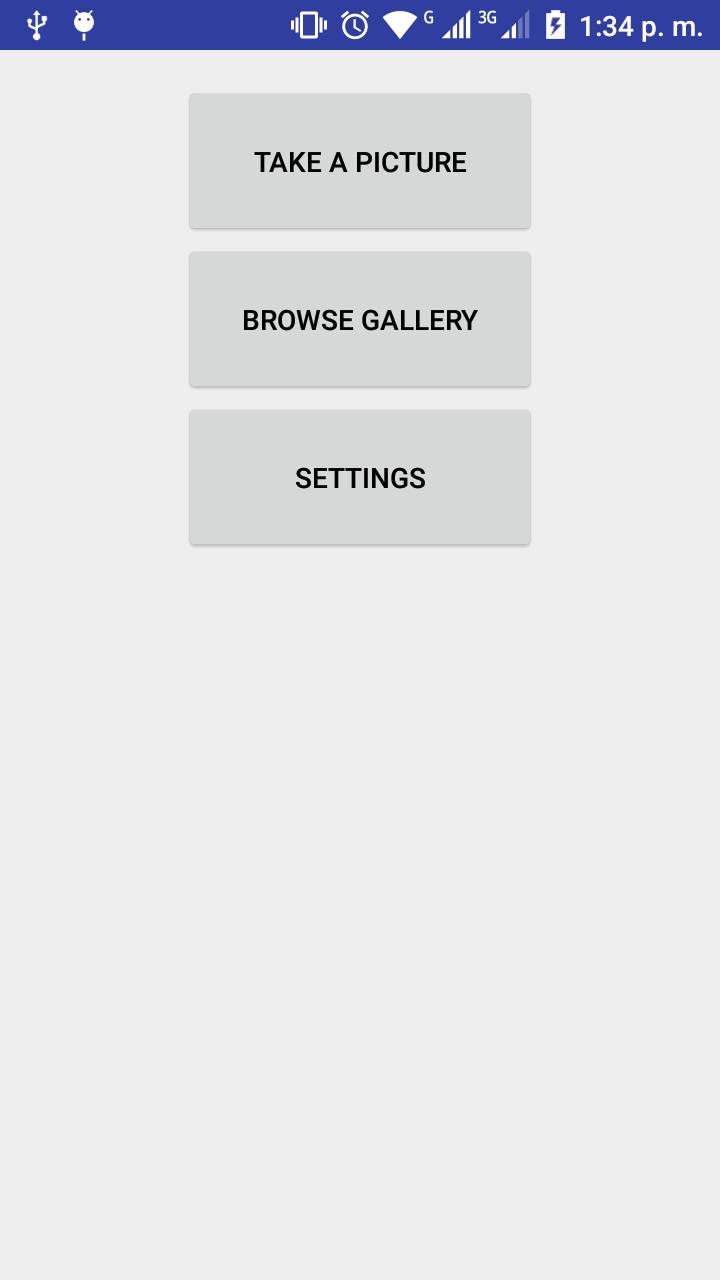
\includegraphics[width=0.4\textwidth]{images/menu}}
			\end{minipage}
			\caption{App - Càmera}
		\end{figure}
		%\begin{figure}[H]
		%	\centering
		%	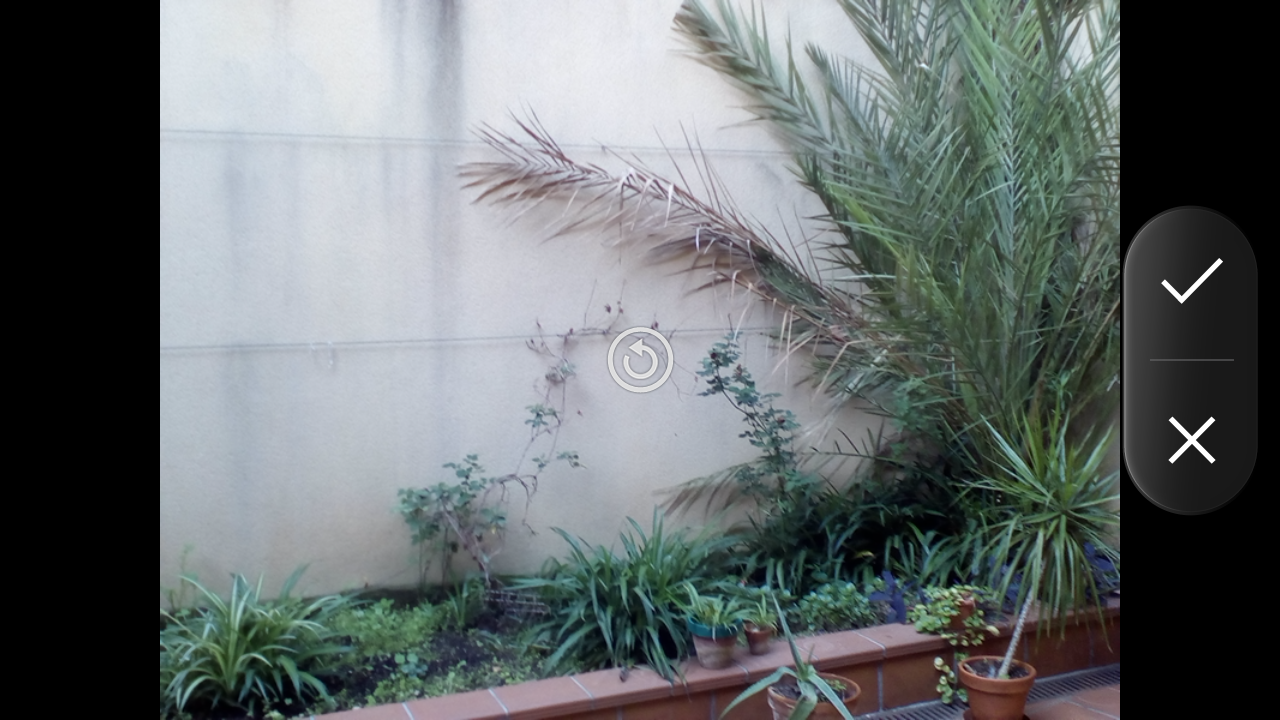
\includegraphics[width=0.5\textwidth]{images/cam}
		%	\caption{App - Càmera}
		%\end{figure}
	\subsubsection{Seleccionar una imatge}
	Si ja es disposa d'una imatge de l'entorn a la memòria del dispositiu, aquesta opció permet a l'usuari seleccionar-la. Un cop realitzada la selecció, l'usuari haurà de seleccionar la regió d'interès.
		\begin{figure}[H]
			\begin{minipage}{6in}
				\centering
				\raisebox{-0.5\height}{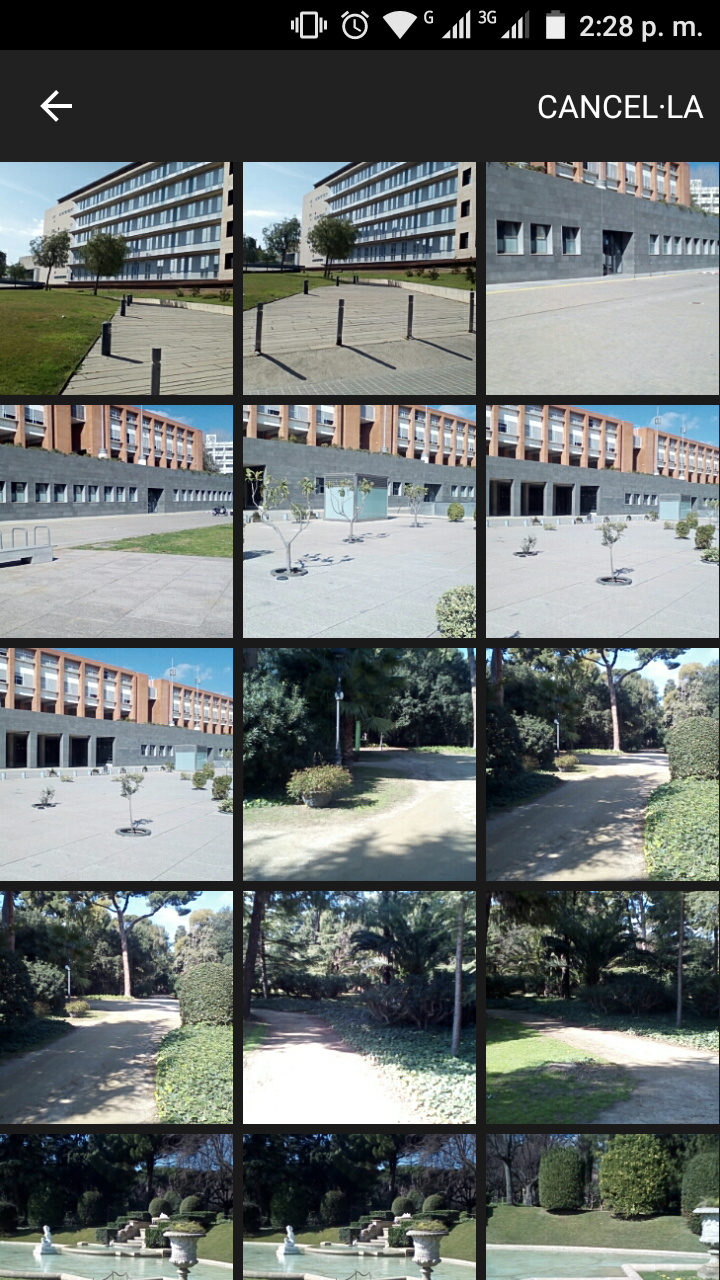
\includegraphics[width=0.4\textwidth]{images/gallery}}
				\hspace*{.2in}
				\raisebox{-0.5\height}{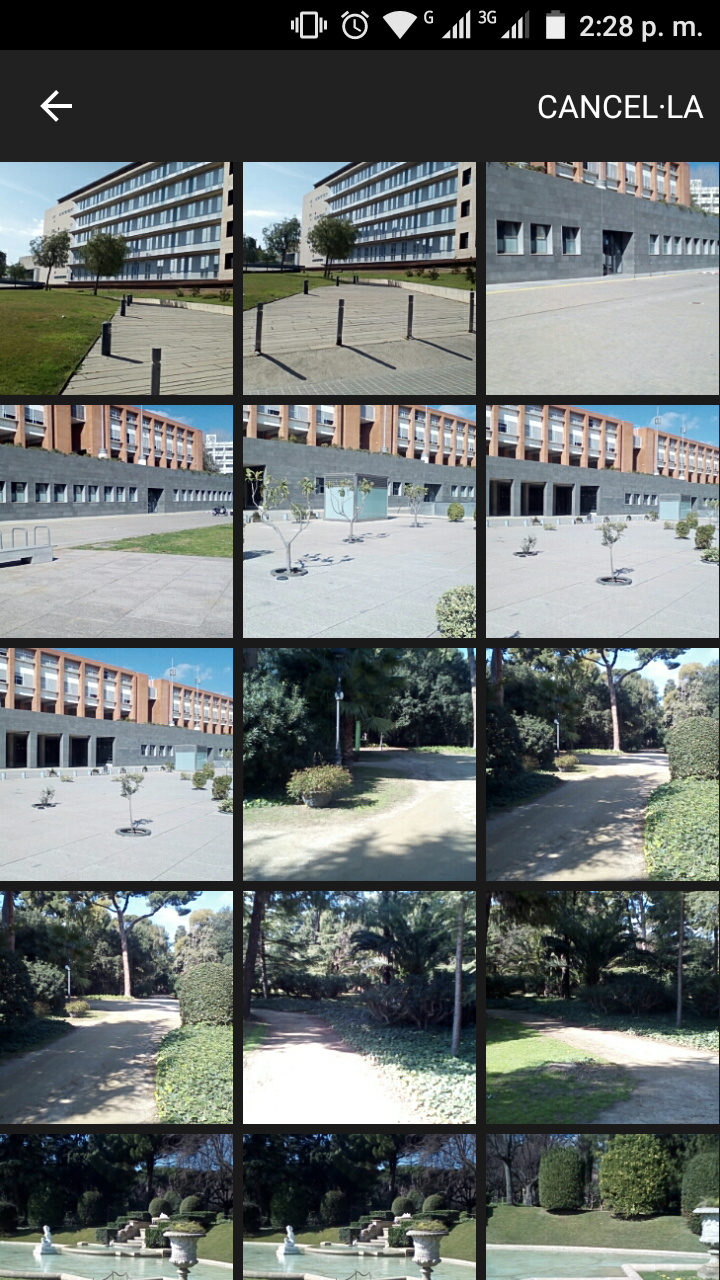
\includegraphics[width=0.4\textwidth]{images/gallery}}
			\end{minipage}
			\caption{App - Galeria}
		\end{figure}
	\subsubsection{Selecció de la regió d'interès}
		Desprès de realitzar una captura o seleccionar una imatge del dispositiu, el programa demanarà a l'usuari que seleccioni una regió d'interès (destí) on vol que es desplaçi el robot.
		\begin{figure}[H]
			\begin{minipage}{6in}
				\centering
				\raisebox{-0.5\height}{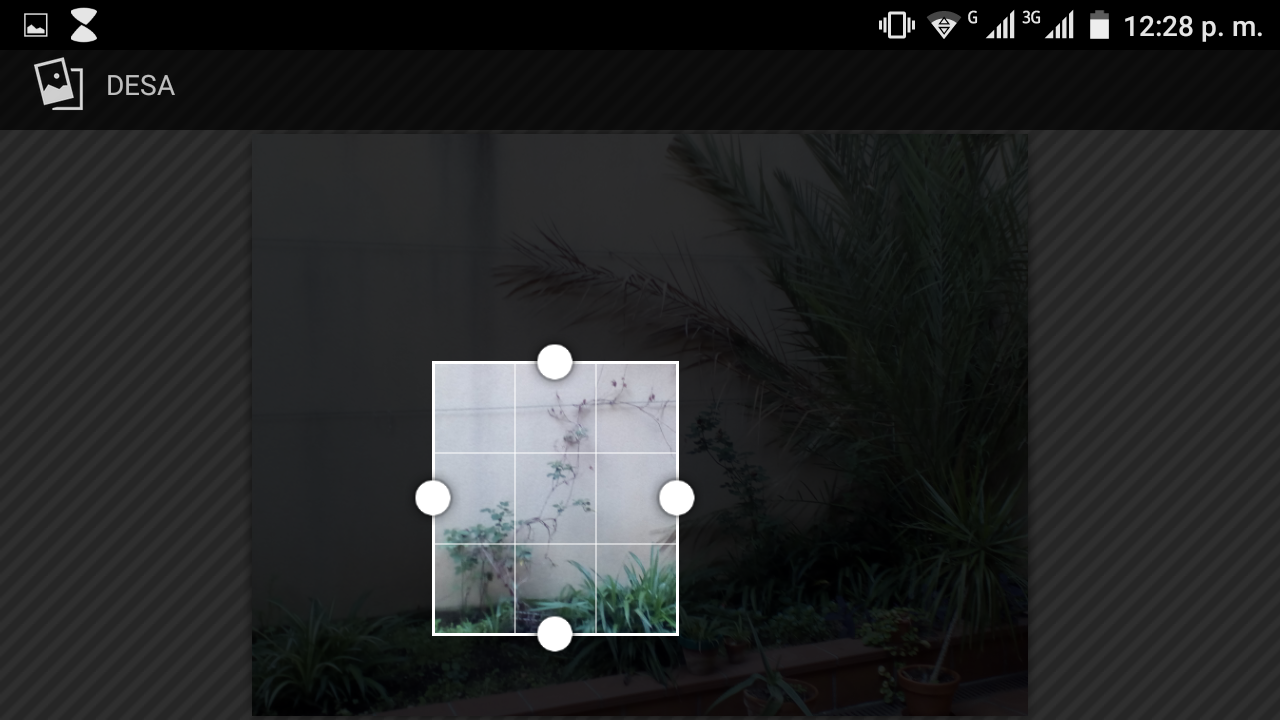
\includegraphics[width=0.4\textwidth]{images/crop}}
				\hspace*{.2in}
				\raisebox{-0.5\height}{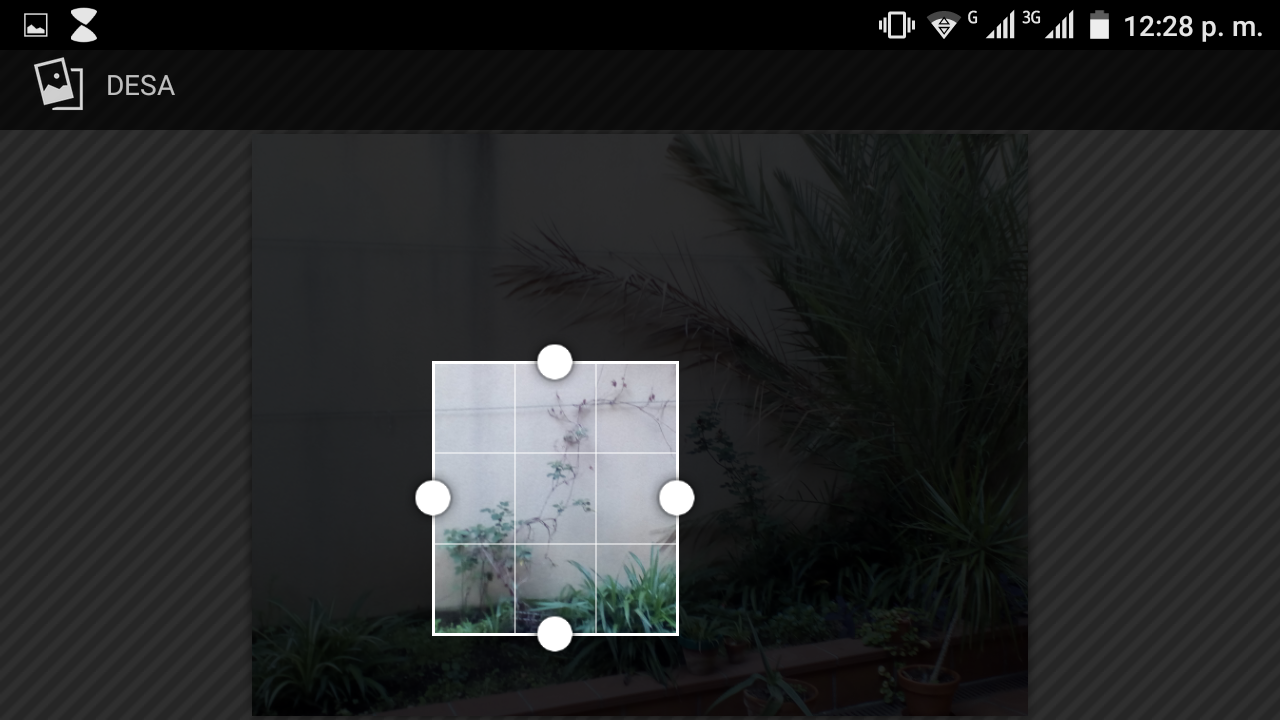
\includegraphics[width=0.4\textwidth]{images/crop}}
			\end{minipage}
			\caption{App - Selecció de la regió d'interès}
		\end{figure}
	\subsubsection{Opcions}
		Des del menú d'opcions, l'usuari hauria de posar les dades per poder connectar-se al robot (direcció IP).\\\\
		I pels usuaris avançats, existeixen opcions per canviar els algorismes de visió per defecte:\\
		\begin{itemize}
			\item{Obtenció de keypoints: Harris, SIFT, SURF, FAST, ORB, BRISK, MSER}
			\item{Extracció de característiques: SIFT, SURF, ORB, BRISK, LATCH, DAISY}
			\item{Homografia: Ransac o asd}
		\end{itemize}
		\begin{figure}[H]
			\begin{minipage}{6in}
				\centering
				\raisebox{-0.5\height}{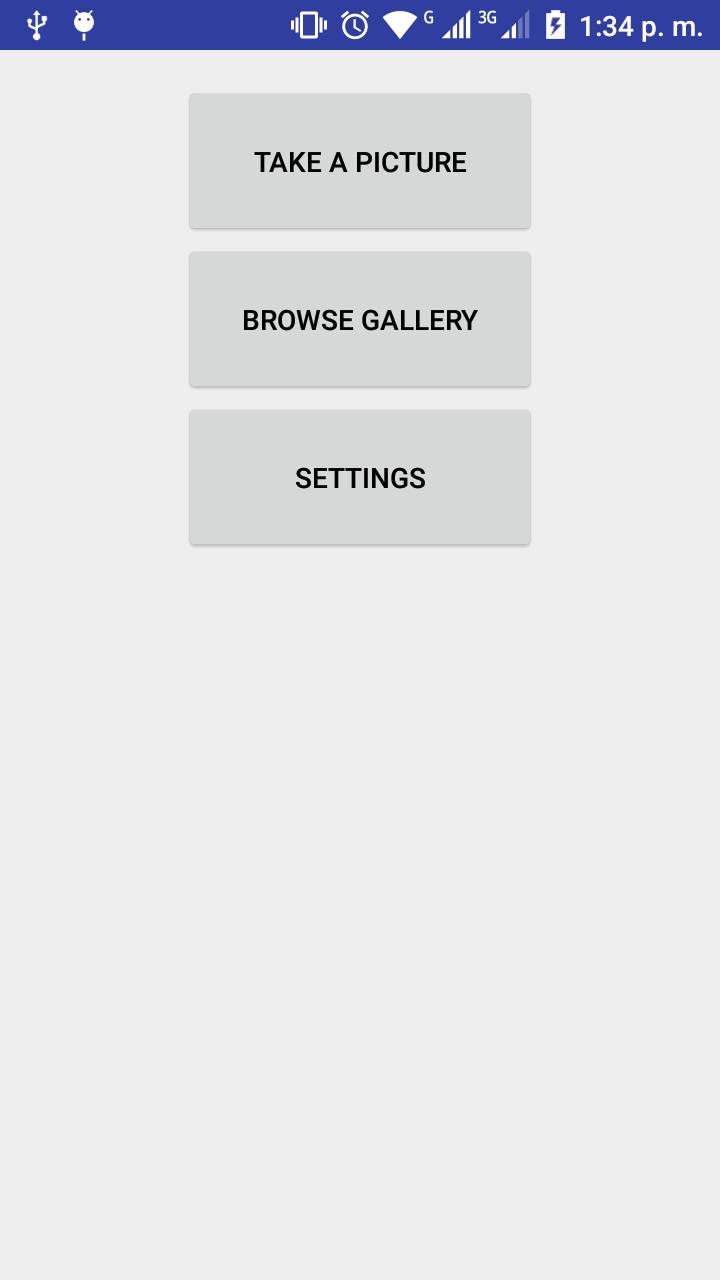
\includegraphics[width=0.4\textwidth]{images/options}}
				\hspace*{.2in}
				\raisebox{-0.5\height}{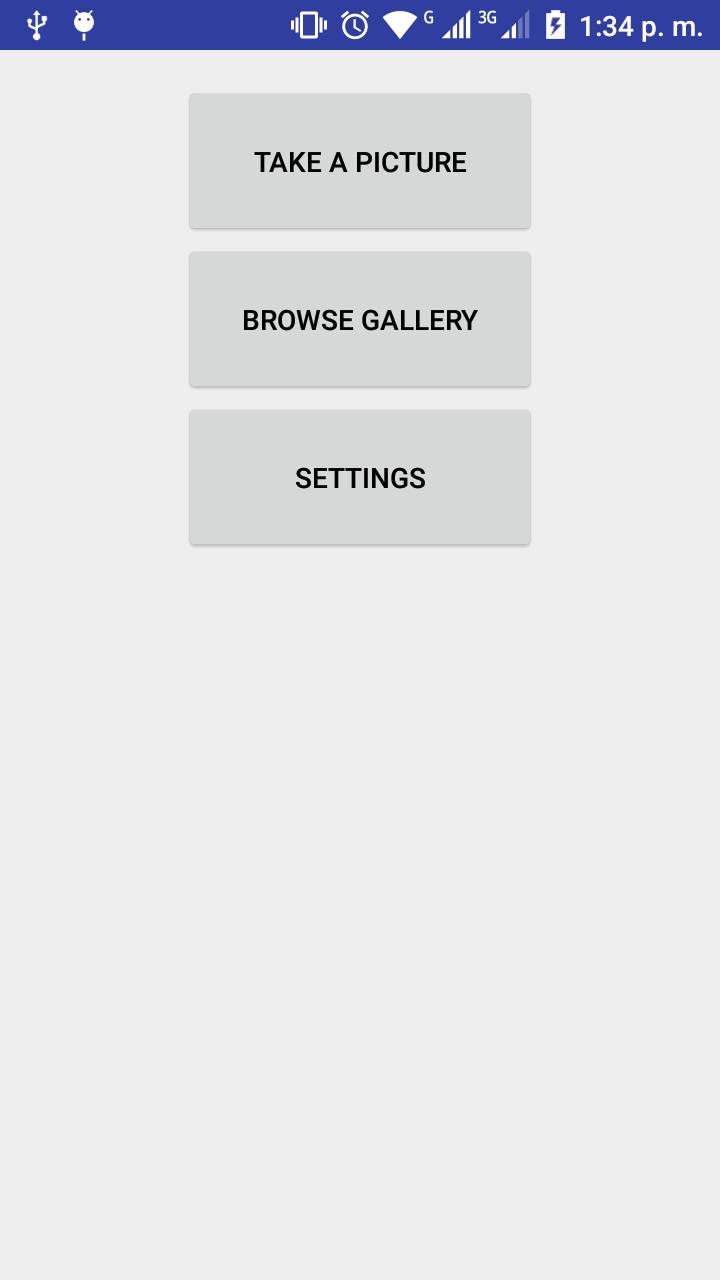
\includegraphics[width=0.4\textwidth]{images/options}}
			\end{minipage}
			\caption{App - Opcions}
		\end{figure}
